% !TEX TS-program = pdflatex
% !TEX encoding = UTF-8 Unicode

% This is a simple template for a LaTeX document using the "article" class.
% See "book", "report", "letter" for other types of document.

\documentclass[11pt]{article} % use larger type; default would be 10pt



%%% The "real" document content comes below...
\usepackage[utf8]{inputenc} % set input encoding (not needed with XeLaTeX)

%%% Examples of Article customizations
% These packages are optional, depending whether you want the features they provide.
% See the LaTeX Companion or other references for full information.

%%% PAGE DIMENSIONS
\usepackage{geometry} % to change the page dimensions
\geometry{a4paper} % or letterpaper (US) or a5paper or....
% \geometry{margin=2in} % for example, change the margins to 2 inches all round
% \geometry{landscape} % set up the page for landscape
%   read geometry.pdf for detailed page layout information

\usepackage{graphicx} % support the \includegraphics command and options

% \usepackage[parfill]{parskip} % Activate to begin paragraphs with an empty line rather than an indent

%%% PACKAGES
\usepackage{booktabs} % for much better looking tables
\usepackage{array} % for better arrays (eg matrices) in maths
\usepackage{paralist} % very flexible & customisable lists (eg. enumerate/itemize, etc.)
\usepackage{verbatim} % adds environment for commenting out blocks of text & for better verbatim
\usepackage{subfig} % make it possible to include more than one captioned figure/table in a single float
% These packages are all incorporated in the memoir class to one degree or another...

%%% HEADERS & FOOTERS
\usepackage{fancyhdr} % This should be set AFTER setting up the page geometry
\pagestyle{fancy} % options: empty , plain , fancy
\renewcommand{\headrulewidth}{0pt} % customise the layout...
\lhead{}\chead{}\rhead{}
\lfoot{}\cfoot{\thepage}\rfoot{}

%%% SECTION TITLE APPEARANCE
\usepackage{sectsty}
\allsectionsfont{\sffamily\mdseries\upshape} % (See the fntguide.pdf for font help)
% (This matches ConTeXt defaults)

%%% ToC (table of contents) APPEARANCE
\usepackage[nottoc,notlof,notlot]{tocbibind} % Put the bibliography in the ToC
\usepackage[titles,subfigure]{tocloft} % Alter the style of the Table of Contents
\renewcommand{\cftsecfont}{\rmfamily\mdseries\upshape}
\renewcommand{\cftsecpagefont}{\rmfamily\mdseries\upshape} % No bold!

%%% END Article customizations
\usepackage{xcolor}
\usepackage{tcolorbox}
\usepackage{lipsum}  % 示例文本
\usepackage{mdframed}

\usepackage{tikz}


\title{Introduction to Math for DS Group Task 0 \\ The Solutions of Three Problems via LLM}
\author{IMDS Group 24 \\ ChatGPT (Zehao Qian) and Bard (Mohammad Jamshaid Iqbal) \\ Bing (Chloe Mendez) annd Answer Analysis (Zeyue Song)}
\begin{document}
\maketitle

\paragraph{\textcolor{red}{Sometimes, a little pre-setting could make GPT's performance better. Below is the first sentence I spoke to ChatGPT:}}

\paragraph{\textcolor{blue}{I'm a data scientist, you're my assistant, I'm having some problems that need mathematical modeling right now, and you're here to assist me.}}

\section{Question 1}
\textcolor{blue}{The air temperature just above the ground at a particular point on the Earth often varies in a periodic manner over a 24 hour cycle. The daily mean value also varies with the seasons over an annual cycle. If we measure time t in hours, what would be an appropriate mathematical model for the temperature as a function of t? }

\begin{mdframed}[
        backgroundcolor=white,  % 背景颜色
        linecolor=black,        % 边框颜色
        leftmargin=5pt,         % 左边距
        rightmargin=5pt,        % 右边距
        linewidth=2pt           % 边框的宽度
    ]
    \textbf{ChatGPT: } establish a mathematical model for the temperature as a function of time, you can consider using trigonometric functions to describe both daily and seasonal variations. Typically, temperature fluctuates in a sinusoidal or cosine-like manner, so you can employ a sine function to model it. Here is a potential model: \par
    \[T(t) = A \sin\left(\frac{2\pi}{24} t + \phi\right) + B\]
    Where:
    - \(T(t)\) represents the temperature at time \(t\).
    - \(A\) is the amplitude, representing the maximum temperature variation.
    - \(t\) is the time in hours.
    - \(\frac{2\pi}{24}\) controls the periodicity, with \(2\pi\) corresponding to a full day (24 hours).
    - \(\phi\) is the phase, indicating the starting point of the temperature within a day.
    - \(B\) is the average temperature, which can vary with the seasons. \par
    You would need to determine the values of the parameters \(A\), \(\phi\), and \(B\) based on actual data. Typically, these parameters can be obtained by fitting the model to historical temperature data. Once you have the appropriate parameters, you can use the model to predict the temperature at any given time. \par
    Please note that this is a simplified model example, and actual situations may be more complex, requiring more data and consideration of factors such as geographical location, elevation, and so on."
\end{mdframed}

\begin{mdframed}[
        backgroundcolor=white,  % 背景颜色
        linecolor=black,        % 边框颜色
        leftmargin=5pt,         % 左边距
        rightmargin=5pt,        % 右边距
        linewidth=2pt           % 边框的宽度
    ]
    \textbf{Bard: } An appropriate mathematical model for the air temperature just above the ground at a particular point on the Earth as a function of time t in hours is: \par
    $$
        T(t) = T_a + T_d \sin(\frac{2 \pi t }{24}) + T_y \sin (\frac{2 \pi t }{365.25})
    $$
    where:
    \begin{itemize}
        \item T(t) is the air temperature at time t in degrees Celsius
        \item $T_a$ is the annual mean temperature in degrees Celsius
        \item $T_d$ is the amplitude of the diurnal temperature variation in degrees Celsius
        \item $T_y$ is the amplitude of the annual temperature variation in degrees Celsius
    \end{itemize}
    The diurnal temperature variation can be modeled using a sinusoidal function with a period of 24 hours. The annual temperature variation can be modeled using a sinusoidal function with a period of 365.25 days. The total temperature is the sum of the annual mean temperature, the diurnal temperature variation, and the annual temperature variation. \par
    The values of $T_a$, $T_d$, and $T_y$ will vary depending on the location on Earth. For example, the annual mean temperature will be higher at the equator than at the poles. The amplitude of the diurnal temperature variation will be greater on clear days than on cloudy days. The amplitude of the annual temperature variation will be greater at higher latitudes than at lower latitudes.
    This model can be used to predict the air temperature at a particular location and time, given the values of $T_a$, $T_d$, and $T_y$. It can also be used to study the effects of climate change on air temperature. \par
\end{mdframed}
% 
% 
\begin{mdframed}[
        backgroundcolor=white,  % 背景颜色
        linecolor=black,        % 边框颜色
        leftmargin=5pt,         % 左边距
        rightmargin=5pt,        % 右边距
        linewidth=2pt           % 边框的宽度
    ]
    \textbf{New Bing: } “The temperature variation over a 24-hour cycle and an annual cycle can be modeled using a trigonometric function. A sinusoidal function can be used to model the temperature variation over a 24-hour cycle, while a cosine function can be used to model the temperature variation over an annual cycle 1.
    A possible mathematical model for the temperature as a function of time t in hours is:
    $$
        T(t) = A sin(2 \pi t/24) + B cos(2 \pi t/365) + C
    $$

    where A, B, and C are constants that depend on the location and other factors 1.
    This model assumes that the temperature variation over a 24-hour cycle is sinusoidal, with a period of 24 hours, and that the temperature variation over an annual cycle is cosine, with a period of 365 days 1.”

\end{mdframed}
% 
% 
% 
\textcolor{blue}{Why use the  trigonometric function to model?}
\begin{mdframed}[
        backgroundcolor=white,  % 背景颜色
        linecolor=black,        % 边框颜色
        leftmargin=5pt,         % 左边距
        rightmargin=5pt,        % 右边距
        linewidth=2pt           % 边框的宽度
    ]
    \textbf{ChatGPT: } The use of a trigonometric function like the sine function in the mathematical model for temperature variations is based on the observation that many natural phenomena, including temperature changes, exhibit periodic behavior that can be described using trigonometric functions. Here's why we use a sine function (which is a type of trigonometric function) in this context:


    \begin{enumerate}
        \item \textbf{Periodicity: }Trigonometric functions, such as sine and cosine, are naturally periodic. They repeat themselves over a regular interval, making them suitable for modeling phenomena that exhibit periodic behavior. In the case of temperature variations, we often see daily and seasonal patterns, both of which are inherently periodic.
        \item \textbf{Smoothness: }Trigonometric functions are smooth and continuous, which makes them a good choice for modeling continuous physical phenomena like temperature changes. They provide a smooth curve that can capture gradual variations in temperature.
        \item \textbf{Amplitude and Phase: }Trigonometric functions have parameters like amplitude (A) and phase (\(\phi\)), which allow us to adjust the height and phase shift of the periodic function. This flexibility enables us to fine-tune the model to fit the specific data we have.
        \item \textbf{Widely Applicable: }Trigonometric functions are widely used in physics and engineering to model periodic phenomena. They have a strong theoretical foundation and have been successfully applied to describe various natural phenomena, including oscillations, waves, and cyclical variations.
        \item \textbf{Empirical Evidence: }Through empirical observation and data analysis, it has been found that temperature variations often follow sinusoidal patterns. Therefore, using a sine function is often a reasonable first approximation.
        \item \textbf{Widely Applicable: }Trigonometric functions are widely used in physics and engineering to model periodic phenomena. They have a strong theoretical foundation and have been successfully applied to describe various natural phenomena, including oscillations, waves, and cyclical variations.
    \end{enumerate}
    While a sine function is a common choice for modeling temperature variations, it's important to note that the actual behavior of temperature can be influenced by numerous factors, and more complex models may be needed to account for additional variables and irregularities in the data. The choice of using a sine function is often a simplification that provides a reasonable starting point for analysis.
\end{mdframed}

\paragraph{\textcolor{red}{Analysis: After analyzing the three answers of Chatgpt, Bard, and Bing, we found that all three models have some things in common. All three answers use trigonometric functions to describe changes in the mathematical model of temperature as a function of time. These three answers are simulated by sine functions. In addition, the three measure “ t ” in hours, so it makes sense to multiply the number of days by the number of hours in a day to keep the graph even. Admittedly, the existence of all three is reasonable, However, when compared, Bard and Bing's answer is better, because ChatGPT's answer does not give a yearly model.}}


\section{Question 2}
\textcolor{blue}{We have a 20 litre bucket that has a hole in the bottom. Every 10 minutes one litre of water flows out of the hole. There is a tap filling the bucket that adds 1 litre of water every 5 minutes. If the bucket starts empty, how long does it take for the bucket to fill?}

\begin{mdframed}[
        backgroundcolor=white,  % 背景颜色
        linecolor=black,        % 边框颜色
        leftmargin=5pt,         % 左边距
        rightmargin=5pt,        % 右边距
        linewidth=2pt           % 边框的宽度
    ]
    \textbf{ChatGPT: } To solve this problem, we can set up an equation to track the net rate at which water enters or leaves the bucket. We know that water flows out of the hole at a rate of 1 liter every 10 minutes and water is added to the bucket at a rate of 1 liter every 5 minutes. Therefore, the net rate of water being added to the bucket is:

    Net rate = (rate of filling) - (rate of draining)

    Net rate = (1 liter per 5 minutes) - (1 liter per 10 minutes)

    Net rate = 0.2 liters per minute - 0.1 liters per minute

    Net rate = 0.1 liters per minute

    This means that every minute, the bucket gains 0.1 liters of water.

    To find out how long it takes for the bucket to fill, we need to figure out how many minutes it will take for the bucket to accumulate 20 liters of water (its capacity).

    Time = (Volume of the bucket) / (Net rate)

    Time = 20 liters / 0.1 liters per minute

    Time = 200 minutes

    So, it will take 200 minutes for the bucket to fill completely.

\end{mdframed}

\begin{mdframed}[
        backgroundcolor=white,  % 背景颜色
        linecolor=black,        % 边框颜色
        leftmargin=5pt,         % 左边距
        rightmargin=5pt,        % 右边距
        linewidth=2pt           % 边框的宽度
    ]
    \textbf{Bard: } Let's assume that the amount of water in the bucket at time t is denoted by V(t). We can then model the rate of change of V(t) using the following equation:
    dV/dt = inflow - outflow

    where:
    inflow is the rate at which water is flowing into the bucket
    outflow is the rate at which water is flowing out of the bucket
    In this case, the inflow is 1 litre per 5 minutes, so we can write:
    inflow = 1/5 litres per minute

    The outflow is 1 litre per 10 minutes, so we can write:
    outflow = 1/10 litres per minute

    Substituting these values into the equation above, we get:
    dV/dt = 1/5 - 1/10 = 1/10 litres per minute

    This equation tells us that the amount of water in the bucket is increasing at a rate of 1/10 litres per minute. We can now use this equation to solve for the time it takes for the bucket to fill.
    To do this, we need to integrate the equation above. This gives us:
    $$
        V(t) = V_0 + (1/10) * t
    $$


    where $V_0$ is the amount of water in the bucket at time t = 0. In this case, the bucket is empty at time t = 0, so $V_0 = 0$.
    We can now set V(t) = 20 litres (the capacity of the bucket) and solve for t:
    20 = 0 + (1/10) * t

    t = 200 minutes

    Therefore, it takes 200 minutes for the bucket to fill.

\end{mdframed}

\begin{mdframed}[
        backgroundcolor=white,  % 背景颜色
        linecolor=black,        % 边框颜色
        leftmargin=5pt,         % 左边距
        rightmargin=5pt,        % 右边距
        linewidth=2pt           % 边框的宽度
    ]
    \textbf{New Bing: }“Let's first calculate the rate at which water is flowing out of the bucket. Since 1 litre of water flows out every 10 minutes, the rate of water flowing out is 0.1 litres per minute.
    Now, let's calculate the rate at which water is flowing into the bucket. Since 1 litre of water is added every 5 minutes, the rate of water flowing in is 0.2 litres per minute.
    Since the rate of water flowing in is greater than the rate of water flowing out, the bucket will eventually fill up. We can use the following formula to calculate how long it takes for the bucket to fill up:
    time = volume / (rate in - rate out)
    where volume is the volume of the bucket, rate in is the rate at which water flows into the bucket, and rate out is the rate at which water flows out of the bucket.
    Substituting the values we calculated earlier, we get:
    time = 20 / (0.2 - 0.1) = 200 minutes
    Therefore, it will take 200 minutes for the bucket to fill up.”
\end{mdframed}


\paragraph{\textcolor{red}{Analysis: ChatGpt, Bard, and Bing give the same answer to this question, and are quite right. But mathematical formulas can never fully reflect the complex reality of the situation, and we need to consider them in terms of real life. For example, we need to take into account that the rate at which water flows out of a bucket is unlikely to be consistent throughout the filling, and that the pressure will increase accordingly. Moreover, the bucket will only fill temporarily, and after this brief equilibrium, it will either overflow if the tap remains open, or empty if the tap is turned off.
    }}

\section{Question 3}
\textcolor{blue}{What is the derivative of $f(x) = 5x(x-1) - 5x^2$?}

\begin{mdframed}[
        backgroundcolor=white,  % 背景颜色
        linecolor=black,        % 边框颜色
        leftmargin=5pt,         % 左边距
        rightmargin=5pt,        % 右边距
        linewidth=2pt           % 边框的宽度
    ]
    \textbf{ChatGPT: } To find the derivative of the function \(f(x) = 5x(x-1) - 5x^2\), you can apply the rules of differentiation. Here's how to do it step by step:

    \begin{enumerate}
        \item Expand the terms within the parentheses: \(f(x) = 5x^2 - 5x - 5x^2\)
        \item Now, differentiate each term separately with respect to \(x\): \\ \(\frac{d}{dx}(5x^2) - \frac{d}{dx}(5x) - \frac{d}{dx}(5x^2)\)
        \item Apply the power rule of differentiation, which states that \(\frac{d}{dx}(x^n) = n x^{n-1}\), where \(n\) is a constant:
        \item Simplify the expression by combining like terms: \(10x - 10x - 5\)
        \item The \(10x\) and \(-10x\) terms cancel each other out, leaving: \(-5\)
    \end{enumerate}
    So, the derivative of the function \(f(x) = 5x(x-1) - 5x^2\) is \(-5\).
\end{mdframed}

\begin{mdframed}[
        backgroundcolor=white,  % 背景颜色
        linecolor=black,        % 边框颜色
        leftmargin=5pt,         % 左边距
        rightmargin=5pt,        % 右边距
        linewidth=2pt           % 边框的宽度
    ]
    \textbf{Bard: } To find the derivative of \(f(x) = 5x(x-1) - 5x^2\), we can use the product rule and the power rule.
    The product rule states that the derivative of the product of two functions u(x) and v(x) is:
    d/dx[u(x)v(x)] = u'(x)v(x) + u(x)v'(x)

    The power rule states that the derivative of $x^n$ is $nx^{n-1}$.
    Let's differentiate f(x) using these rules:
    $$
        f'(x)=\frac{d}{dx}[5x(x-1) - 5x^2]
    $$
    Therefore, the derivative of f(x) is $10x - 5$.

\end{mdframed}

\begin{mdframed}[
        backgroundcolor=white,  % 背景颜色
        linecolor=black,        % 边框颜色
        leftmargin=5pt,         % 左边距
        rightmargin=5pt,        % 右边距
        linewidth=2pt           % 边框的宽度
    ]
    \textbf{New Bing: }“The derivative of the function $f(x) = 5x(x-1) - 5x^2$ can be calculated using the product rule and the power rule of differentiation.
    The product rule states that if f(x) = u(x) * v(x), then f'(x) = u'(x) * v(x) + u(x) * v'(x).
    Using the product rule, we get:
    $f'(x) = (5x)'(x-1) + 5x(x-1)' - (5x^2)$'
    Applying the power rule, we get:
    f'(x) = (5(x-1)) + 5x(1) - (10x)
    Simplifying, we get:
    f'(x) = 5x - 5
    Therefore, the derivative of $f(x)$ is $f'(x) = 5x - 5$.”
\end{mdframed}

\paragraph{\textcolor{red}{Analysis: ChatGPT's answer is correct, Bard and Bing both give the wrong answer. We think that the product rule should not be used in this problem, but the rules of differentiation should be applied. Because in this case the expression is not expanded, and there is an addition after the multiplication. Therefore, ChatGpt's answer is the correct one.}}
% 
% 
% 
% 
% 
% 
% 
% 
% 
% 



\tikzset{every picture/.style={line width=0.75pt}} %set default line width to 0.75pt        

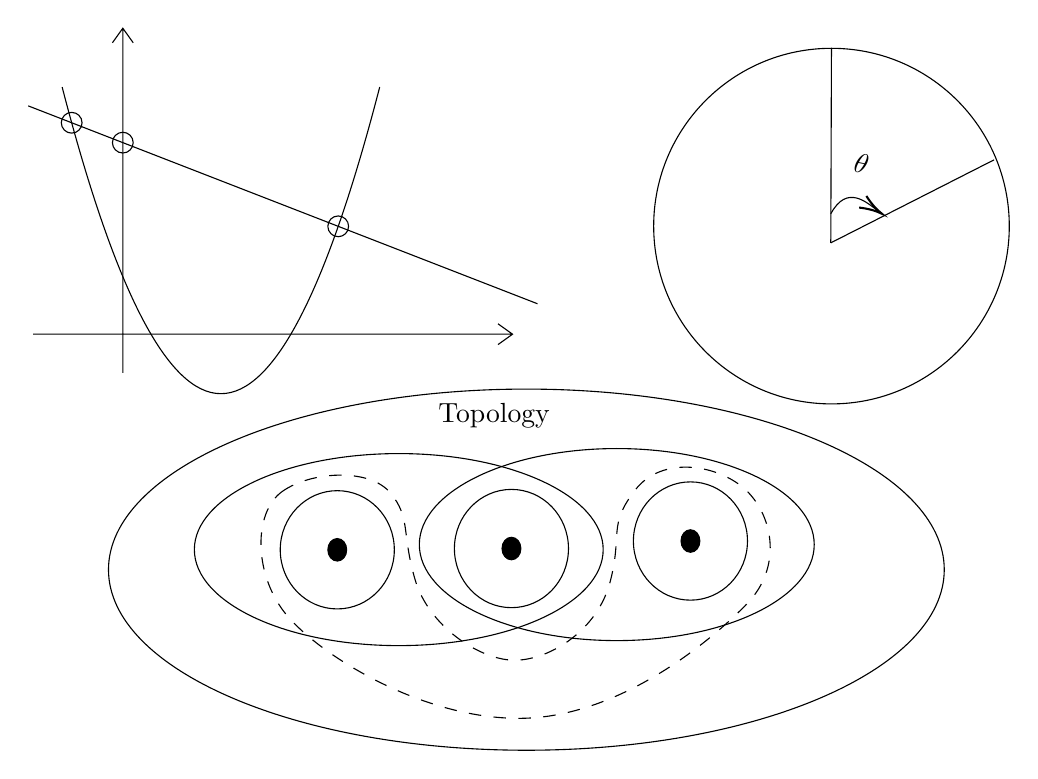
\begin{tikzpicture}[x=0.75pt,y=0.75pt,yscale=-1,xscale=1]
    %uncomment if require: \path (0,365); %set diagram left start at 0, and has height of 365

    %Shape: Axis 2D [id:dp3330650107827038] 
    \draw  (52.67,153.74) -- (283.67,153.74)(95.9,6.33) -- (95.9,172.41) (276.67,148.74) -- (283.67,153.74) -- (276.67,158.74) (90.9,13.33) -- (95.9,6.33) -- (100.9,13.33)  ;
    %Shape: Parabola [id:dp6747224874888704] 
    \draw   (66.67,34.67) .. controls (117.67,231.65) and (168.67,231.65) .. (219.67,34.67) ;
    %Straight Lines [id:da4045208158970277] 
    \draw    (50.33,43.74) -- (295.67,139.07) ;
    %Shape: Circle [id:dp9495260244967654] 
    \draw   (351.67,101.67) .. controls (351.67,54.35) and (390.02,16) .. (437.33,16) .. controls (484.65,16) and (523,54.35) .. (523,101.67) .. controls (523,148.98) and (484.65,187.33) .. (437.33,187.33) .. controls (390.02,187.33) and (351.67,148.98) .. (351.67,101.67) -- cycle ;
    %Straight Lines [id:da6440917457226727] 
    \draw    (437.33,16) -- (437,109.74) ;
    %Straight Lines [id:da2506243181764847] 
    \draw    (515.67,69.74) -- (437,109.74) ;
    %Curve Lines [id:da36631824919286937] 
    \draw    (437,95.74) .. controls (444.89,81.18) and (454.43,90.36) .. (460.1,94.64) ;
    \draw [shift={(461.67,95.74)}, rotate = 212.01] [color={rgb, 255:red, 0; green, 0; blue, 0 }  ][line width=0.75]    (10.93,-3.29) .. controls (6.95,-1.4) and (3.31,-0.3) .. (0,0) .. controls (3.31,0.3) and (6.95,1.4) .. (10.93,3.29)   ;
    %Shape: Ellipse [id:dp9329672718104849] 
    \draw   (89,267.19) .. controls (89,219.14) and (179.14,180.19) .. (290.33,180.19) .. controls (401.53,180.19) and (491.67,219.14) .. (491.67,267.19) .. controls (491.67,315.24) and (401.53,354.19) .. (290.33,354.19) .. controls (179.14,354.19) and (89,315.24) .. (89,267.19) -- cycle ;
    %Shape: Ellipse [id:dp9998724111128214] 
    \draw   (130.37,257.52) .. controls (130.37,231.97) and (174.47,211.26) .. (228.86,211.26) .. controls (283.25,211.26) and (327.34,231.97) .. (327.34,257.52) .. controls (327.34,283.08) and (283.25,303.79) .. (228.86,303.79) .. controls (174.47,303.79) and (130.37,283.08) .. (130.37,257.52) -- cycle ;
    %Shape: Ellipse [id:dp6415322670258081] 
    \draw   (238.76,255.11) .. controls (238.76,229.56) and (281.35,208.84) .. (333.89,208.84) .. controls (386.43,208.84) and (429.02,229.56) .. (429.02,255.11) .. controls (429.02,280.66) and (386.43,301.37) .. (333.89,301.37) .. controls (281.35,301.37) and (238.76,280.66) .. (238.76,255.11) -- cycle ;
    %Shape: Ellipse [id:dp6607583700307356] 
    \draw   (171.75,257.62) .. controls (171.75,241.88) and (184.05,229.13) .. (199.23,229.13) .. controls (214.4,229.13) and (226.71,241.88) .. (226.71,257.62) .. controls (226.71,273.35) and (214.4,286.11) .. (199.23,286.11) .. controls (184.05,286.11) and (171.75,273.35) .. (171.75,257.62) -- cycle ;
    %Shape: Ellipse [id:dp7853319365959068] 
    \draw   (255.66,257.01) .. controls (255.66,241.28) and (267.96,228.52) .. (283.14,228.52) .. controls (298.32,228.52) and (310.62,241.28) .. (310.62,257.01) .. controls (310.62,272.75) and (298.32,285.5) .. (283.14,285.5) .. controls (267.96,285.5) and (255.66,272.75) .. (255.66,257.01) -- cycle ;
    %Shape: Ellipse [id:dp5078229765284272] 
    \draw   (341.9,253.39) .. controls (341.9,237.65) and (354.21,224.9) .. (369.38,224.9) .. controls (384.56,224.9) and (396.86,237.65) .. (396.86,253.39) .. controls (396.86,269.12) and (384.56,281.88) .. (369.38,281.88) .. controls (354.21,281.88) and (341.9,269.12) .. (341.9,253.39) -- cycle ;
    %Shape: Ellipse [id:dp47882141993434524] 
    \draw  [fill={rgb, 255:red, 0; green, 0; blue, 0 }  ,fill opacity=1 ] (364.85,253.39) .. controls (364.85,250.4) and (366.88,247.97) .. (369.38,247.97) .. controls (371.89,247.97) and (373.92,250.4) .. (373.92,253.39) .. controls (373.92,256.38) and (371.89,258.81) .. (369.38,258.81) .. controls (366.88,258.81) and (364.85,256.38) .. (364.85,253.39) -- cycle ;
    %Shape: Polygon Curved [id:ds8181656794178567] 
    \draw  [dash pattern={on 4.5pt off 4.5pt}] (172.76,229.48) .. controls (186.67,219.68) and (214.76,218.15) .. (224.76,230.15) .. controls (234.76,242.15) and (230.1,249.48) .. (236.76,272.15) .. controls (243.43,294.82) and (268.63,311.28) .. (285.43,310.82) .. controls (302.23,310.35) and (324.76,296.15) .. (330.76,272.82) .. controls (336.76,249.48) and (329.43,246.15) .. (342.76,228.82) .. controls (356.1,211.48) and (384.1,216.82) .. (396.76,229.48) .. controls (409.43,242.15) and (413.43,266.15) .. (396.76,283.48) .. controls (380.1,300.82) and (335.47,338.48) .. (287.43,338.82) .. controls (239.39,339.16) and (189.43,307.48) .. (174.1,288.15) .. controls (158.76,268.82) and (158.86,239.29) .. (172.76,229.48) -- cycle ;
    %Shape: Ellipse [id:dp26952850031511955] 
    \draw  [fill={rgb, 255:red, 0; green, 0; blue, 0 }  ,fill opacity=1 ] (278.6,257.01) .. controls (278.6,254.02) and (280.63,251.59) .. (283.14,251.59) .. controls (285.65,251.59) and (287.68,254.02) .. (287.68,257.01) .. controls (287.68,260.01) and (285.65,262.43) .. (283.14,262.43) .. controls (280.63,262.43) and (278.6,260.01) .. (278.6,257.01) -- cycle ;
    %Shape: Ellipse [id:dp7070111192051278] 
    \draw  [fill={rgb, 255:red, 0; green, 0; blue, 0 }  ,fill opacity=1 ] (194.69,257.62) .. controls (194.69,254.62) and (196.72,252.2) .. (199.23,252.2) .. controls (201.73,252.2) and (203.76,254.62) .. (203.76,257.62) .. controls (203.76,260.61) and (201.73,263.04) .. (199.23,263.04) .. controls (196.72,263.04) and (194.69,260.61) .. (194.69,257.62) -- cycle ;

    % Text Node
    \draw (448.84,64.99) node [anchor=north west][inner sep=0.75pt]  [rotate=-12,xslant=0.03]  {$\theta $};
    % Text Node
    \draw (246.67,185.63) node [anchor=north west][inner sep=0.75pt]   [align=left] {Topology};

    \draw   (95.9, 61.45) circle [x radius= 5, y radius= 5]   ;
    \draw   (199.68, 101.77) circle [x radius= 5, y radius= 5]   ;
    \draw   (71.26, 51.87) circle [x radius= 5, y radius= 5]   ;
\end{tikzpicture}
% 
% 
% 
% 
% 
% 
% 
% 
% 
% 
\end{document}
